%================================================================
\section{Theory}\label{sec:Theory}
%================================================================


%----------------------------------------------------------------
\subsection{System}\label{sec:systems}
%----------------------------------------------------------------

We will be considering two system : one electron in a one-dimensional harmonic oscillator trap, and two electrons interacting via the Coulomb interactions in a two-dimensional isotropic harmonic oscillator trap.

A general idealized Hamiltonian for $N$ interacting particles in a $d$-dimensional isotropic trap is given by 
\begin{equation}
    H = \sum_{i=1}^N \qty(-\frac{1}{2}\laplacian_i+ \frac{1}{2}\omega^2 \bm{r_i}\cdot\bm{r_i}) + \sum_{i<j}\frac{1}{r_{ij}}, 
\end{equation}
where we are using the natural units given by $\hbar=c=e=m_e=k_e=1$, $\bm{r}_i\cdot\bm{r}_i$ denotes the dot product of the positions of particle $i$, and all the energies are in atomic units (a.u), and $D$ is the dimensionality of the trap. The kinetic energy of the electrons is given $\sum_{i=1}^N\qty(-\frac{1}{2}\laplacian_i)$, the potential energy with respect to the trap potential is given $\sum_{i=1}^N \qty(\frac{1}{2}D\omega^2r_i^2)$, and the Coulomb interactions are modeled as the inverse Euclidian distance between the electrons ($r_{ij} = \norm{\bm{r}_i-\bm{r}_j}_2$). Notice that $\sum_{i<j}$ denotes a double sum, such that 
\begin{equation}
    \sum_{i<j}\frac{1}{r_{ij}} = \sum_{i=1}^{N-1}\sum_{j=i+1}^N\frac{1}{r_{ij}}. 
\end{equation}
We denote the non-interacting part of the Hamiltonian $H_0$ and the Coulomb interaction $H_1$, such that for an interacting system we get $H = H_0 + H_1$. For the system of a single particle in the one-dimensional harmonic oscillator trap, the Hamiltonian becomes
\begin{equation}\label{eq:1dHamiltonian}
    H = -\frac{1}{2}\laplacian + \frac{1}{2}\omega^2 x^2, 
\end{equation}
where $x$ denotes the coordinate with respect to the center of the trap. The general eigenstate of the 1D Hamiltonian is given by  
\begin{equation}
    \phi_n = AH_n\qty(\sqrt{\omega}x)\exp{-\omega x^2/2}, 
\end{equation}
where $A$ is a normalization constant, $H_n\qty(\sqrt{\omega}x)$ are the Hermite polynomials with respect to the quantum number $n$. The corresponding energy eigenvalue of the eigenstate is $E_n = \omega\qty(n + \frac{1}{2})$ a.u. The ground state of this system occurs when $n=0$, and is given as 
\begin{equation}
    \phi_0 = A\exp{-\omega x^2}, 
\end{equation}
where $A = \qty(\frac{\omega}{\pi})^{\frac{1}{4}}$ is such that $\braket{\phi_0} = \int_{x\in\mathbb{R}}\abs{\phi_0}^2\mathrm{d}x = 1$. The energy of the ground state is $E_0 = \omega\frac{1}{2}$ a.u. 

The system of two Coulomb interacting particles in a two-dimensional isotropic harmonic oscillator trap, has the Hamiltonian 
\begin{equation}\label{eq:2dHamiltonian}
    H = -\frac{1}{2}\qty(\laplacian_1 + \laplacian_2) + \frac{\omega^2}{2}\qty(\bm{r}_1\cdot\bm{r}_1 + \bm{r}_2\cdot\bm{r}_2) + \frac{1}{r_{12}}, 
\end{equation}
and its analytical ground state energy $E_0$ is $3$ a.u., shown in \citep{PhysRevA.48.3561}. The non-interacting part of the Hamiltonian has the analtyical eigenstate 
\begin{equation}
    \phi_{n_x,n_y}(x,y) = A H_{n_x}(\sqrt{\omega}x)H_{n_y}(\sqrt{\omega}y)\exp{(-\omega(x^2+y^2)/2)}, 
\end{equation}
with the corresponding energy eigenvalue of 
\begin{equation*}
    E_{n_x, n_y} = \omega\qty(n_x + n_y + 1), 
\end{equation*}
which yields the ground state $n_x = n_y = 0$, $E_{0, 0}=\omega$. The two electrons can have the same quantum numbers due to their spin quantum number being different, which does not affect the energy. However, if there are more electrons, the wave functions need to take into account that two fermions cannot occupy the same quantum numbers. We say that the degeneracy of the ground state wave function for the harmonic oscillator is two. 


\subsection{Neural Networks}
Artificial Neural Networks, or simply just Neural Networks (NN), are computer systems which are modeled after the biological neural networks of animal brains. Just like biological brains, Neural Networks consists of neurons which either activate or or not depending on if a given threshold is reached. Each connection of a Neural Network can be compared with the synapses of a biological brain. They transmit signals to other neurons. However, biological neural networks learn through a process called synaptic plasticity, while artificial while learn by adjusting it's weights and biases in order to minimize a given cost function. The weights of the Neural Network are the connections between two neurons. In Graph Theory, we would refer to them as (weighted) edges between nodes. The bias term shifts the input of a neuron. The general approach to neural networks is to train it using gradients of a \textit{cost function}, i.e. a distance between the ground truth labels and the prediction yielded. Then perform a gradient-based approach to update the parameters of the neural network. 
\\
A Neural Network consists of an input layer, a hidden layer, or multiple hidden layers as in the case of deep neural networks, and an output layer. An example of a neural network architecture with three hidden layers and three outputs is displayed in \autoref{fig:NN}. %[\textcolor{blue}{Figure 1}]

\begin{figure}[htbp]
  \centering
  %\includesvg[scale= 0.4]{Images/Neural-Network.svg}
  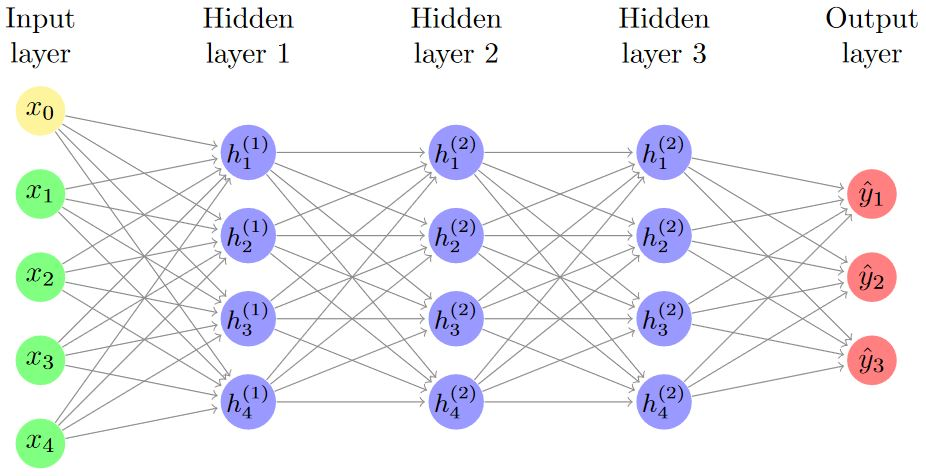
\includegraphics[scale=0.5]{Images/DFFNN.JPG}
  \caption{Wrong! A simple Feed-forward Neural Network with 3 input neurons, 1 output neuron and 3 layers of hidden layers consisting of 4 neurons each.$x_0$ is the bias term}
  \label{fig:NN}
\end{figure}

Generally, we can group machine learning in three general categories; supervised and unsupervised learning. If you have a data set $\mathcal{D}$ with known ground truth labels and train the neural network to learn a function for the features of the network that produces a general output equal that corresponds well to a general data set of same distribution as $\mathcal{D}$, we have supervised learning. Unsupervised learning takes a data set without known ground truth labels and tries to find correlations between the data. Reinforcement learning is performed when we do not have ground truth labels and use some kind of other measure to find a probability distribution to match. The measure can for example be the predicted labels of another well-trained network, or a principle. In our case we train the network based on the variational principle (see \citep{project1}), which states that any approximation to the expectation value of energy is greater or equal to the ground state energy. 

%----------------------------------------------------------------
\subsection{Boltzmann machines}
%----------------------------------------------------------------
A \textit{Boltzmann machine} (BM) is an undirected probabilistic graphical model with stochastic continuous or discrete nodes. It consists of one visible and one hidden layer, which are both inter- and intraconnected, meaning that there are weight matrices that represents the strength of the interactions between the nodes (both within the same layer and connections to the nodes in the other layer). The Boltzmann machine is a generative model as it allows generating new samples from a learned distribution. These properties are useful in our search for a ground state wave function, however, the Boltzmann machine requires a large computational cost to train. We will therefore employ a \textit{restricted Boltzmann machine} to do our bidding.  \autoref{fig:vis_BM} is a simple representation of a BM network, where all the nodes are connected. 

\begin{figure}[H]
\begin{center}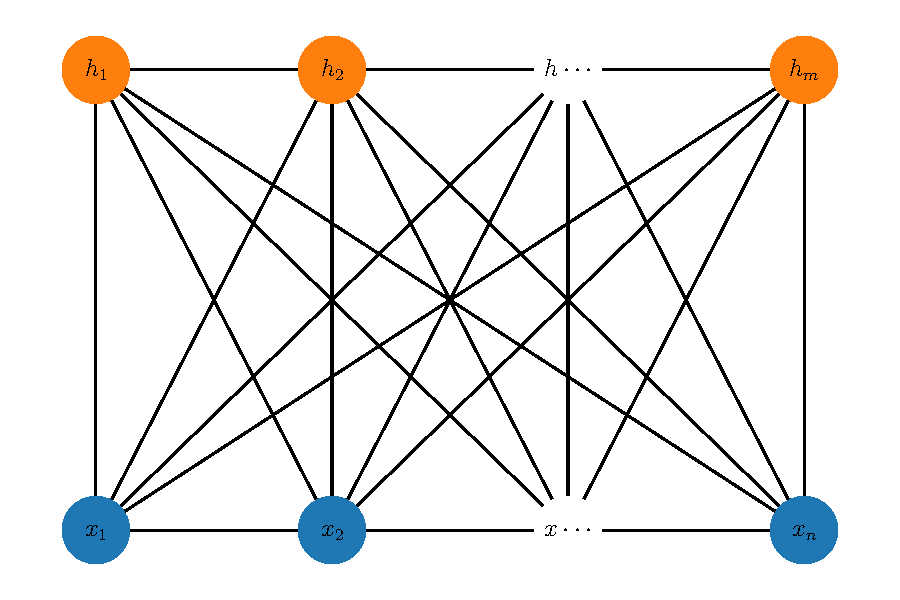
\includegraphics[scale=0.8]{latex/latex-report/Images/bm_visualize.pdf}
\end{center}
\caption{Simple visualization of a BM network with a visible layer of $n$ nodes and a hidden layer of $m$ nodes. The links between the nodes are weighted, and they are all contained within a weight matrix, $W$. The BM network is fully connected between all nodes. Every link is undirected, as the connections go both ways.}
\label{fig:vis_BM}
\end{figure}

%----------------------------------------------------------------
\subsection{Restricted Boltzmann Machines}
%----------------------------------------------------------------
The visible and hidden layer of the RBM is interconnected, but not intraconnected. The connections between the hidden layer, $\bm{h}\in\mathbb{R}^N$, and the visual layer, $\bm{x}\in\mathbb{R}^M$, are weighted by the weight matrix $W\in\mathbb{R}^{M\times N}$, represented by the edges in \autoref{fig:vis_RBM}. The layers can both have biases of equal length. We denote the bias for the visible layer, $\bm{a}$, and for the hidden layer, $\bm{b}$. 
The most common type of an RBM is the \textit{binary-binary RBM}, but to be able to represent the continuous configuration space of the particles, we will use a \textit{Gaussian-binary RBM}. 


\begin{figure}[H]
\begin{center}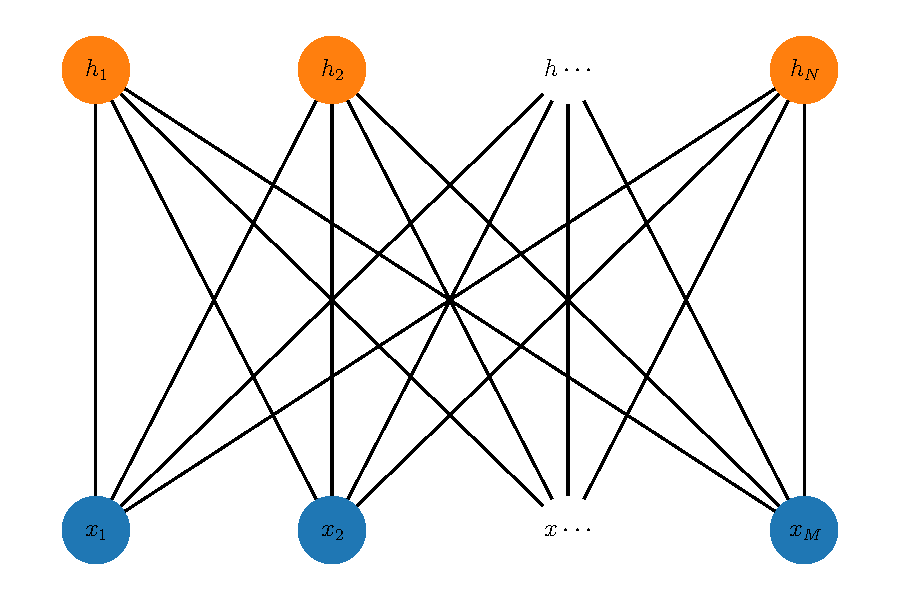
\includegraphics[scale=0.8]{latex/latex-report/Images/rbm_visualize.pdf}
\end{center}
\caption{Simple visualization of an RBM network with a visible layer of $n$ nodes and hidden layer layer of $m$ nodes. The links between the nodes are weighted, and they are all contained within a weight matrix, $W$. The RBM network is fully connected between the layers. Every link is undirected, as the connections go both ways.}
\label{fig:vis_RBM}
\end{figure}

%----------------------------------------------------------------
\subsubsection{Representing the wave function using a neural network.}
%----------------------------------------------------------------
Approximating a high dimensional wave function to a high degree of certainty requires a large computational cost, and often becomes practically intractable for large system. We want an RBM to learn the wave function (our system has a wave function fully defined in the real domain) of the quantum mechanical system we want to simulate, and generate samples using the RBM as our system. The RBM representation of the wave function was first done by \citep{Carleo_2017} and they coined the general approximation of a wave function using a neural network method a \textit{neural network quantum state}, or NQS. When applied to large system of particles, the NQS may offer a lower computational cost compared with traditional methods. %However, we will try to use the an NQS to solve the systems explained in \autoref{sec:systems}

The Boltzmann distribution describes the probability of a system being in a certain state as a function of energy and temperature. It is widely used in statistical physics and mathematics. Mathematically, it can be stated as 
\begin{equation}\label{eq:boltzmann_dist}
    p_i = \frac{e^{-\frac{1}{T}E_i}}{Z}, 
\end{equation}
where $E_i$ is the energy of state $\ket{i}$, $T$ is the `temperature' of the system and $Z$ denotes the \textit{partition function}. The partition function has the form
\begin{equation*}
    Z = \sum_{j=0}^{J-1} e^{-\frac{1}{T}E_j}, 
\end{equation*}
where $J$ is the number of possible states, and is the normalization condition for the probability $p_i$. Now, if we define the \textit{energy function} of the neural network to be a function of the visible and hidden layers, $E\qty(\bm{x}, \bm{h})$, we can use the Boltzmann distribution to define a joint probability function 
\begin{equation}\label{eq:joint_probability}
    p\qty(\bm{x}, \bm{h}) = \frac{e^{-\frac{1}{T}E\qty(\bm{x}, \bm{h})}}{Z}.
\end{equation}
The partition function, $Z$, will then be the sum of all possible configurations of visible and hidden nodes, 
\begin{equation}\label{eq:partition_function}
    Z = \int\int e^{-\frac{1}{T}E\qty(\bm{x}, \bm{h})}\mathrm{d}\bm{x}\mathrm{d}\bm{h}.
\end{equation}
Generally, calculating the partition function is intractable (or just inconvenient), and is luckily not needed. The reason is that we use Markov chain Monte Carlo (MCMC) methods that only need the \textit{ratio} between states to generate new samples for the chain. To see this, say $p = p(\bm{x}, \bm{h})$ is the joint probability for state $\bm{x}$ and $p' = p\qty(\bm{x'},\bm{h})$ is the joint probability for state $\bm{x'}$, we get the ratio 
\begin{equation*}
    \frac{p'}{p} = \exp{-\frac{1}{T}E\qty(\bm{x'}, \bm{h}) + \frac{1}{T}E\qty(\bm{x}, \bm{h})}. 
\end{equation*}
Further, we will set the `temperature' parameter equal to 1. 
%----------------------------------------------------------------
\subsection{Gaussian-Binary RBM}
%----------------------------------------------------------------
The Gaussian-Binary RBM can represent continuous configuration space, such as our systems. Another advantage it has, is that the Gaussian part of the wave function can easily be approximated by the Gaussian part of the RBM, and thus it should be a suitable choice of wave function. The energy function $E\qty(\bm{x}, \bm{h})$, is given as 
\begin{equation*}
    E\qty(\bm{x}, \bm{h}) = \sum_i^M \frac{(x_i - a_i)^2}{2\sigma_i^2} - \sum_j^N b_j h_j - \sum_{i,j}^{M,N} \frac{x_i w_{ij} h_j}{\sigma_i^2} 
\end{equation*}
or, in vector notation, as 
\begin{equation}\label{eq:energy_function_RBM}
    E\qty(\bm{x}, \bm{h}) = \frac{\norm{\bm{x}-\bm{a}}^2}{2\sigma^2} - \bm{b}^T\bm{h} - \frac{\bm{x}\bm{W}\bm{h}}{\sigma^2}. 
\end{equation}
$\sigma^2$ will refer to the expected variance in the Gaussian layer of the model, which will be treated as a hyper parameter in this project. 

%----------------------------------------------------------------
\subsection{Optimizing the RBM}
%----------------------------------------------------------------
We will treat the expectation value of the local energy as the cost function of our RBM and try and minimize it, as according to the variational principle. 

%----------------------------------------------------------------
\subsubsection{Derivations of local energy.}
%----------------------------------------------------------------

We want the NQS marginal probability distribution over the visible layer to mimic the wave function (alternatively, the square of the wave function). Therefore, 
\begin{equation*}
    p(\bm{x}) = \sum_{j=1}^N \frac{\mathrm{e}^{-\frac{1}{T}E\qty(\bm{x}, \bm{h})}}{Z}, 
\end{equation*}
will act as our trial wave function, $\Psi_T(\bm{x})$. For a Gaussian-Binary RBM, the marginal PDF can be expanded into
\begin{equation*}
    \Psi_T(\bm{x}) = \frac{\mathrm{e}^{-\frac{\norm{\bm{x}-\bm{a}}^2}{2\sigma^2}}}{Z}\prod_j^N \qty(1 + \mathrm{e}^{b_j + \qty[\frac{\bm{x}}{\sigma^2}]^T W_{*j}}). 
\end{equation*}
To compute the kinetic energy of the system ($K$), we will apply the formula 
\begin{equation*}
    K = -\frac{1}{2}\sum_i^M \qty(\qty(\pdv{\ln{\Psi}}{x_i})^2 + \pdv[2]{\ln{\Psi}}{x_i}), 
\end{equation*}
which is derived in \citep{project1}. The trial wave function in the logarithmic domain is 
\begin{equation*}
    \ln{\Psi_T\qty(\bm{x})} = -\frac{\norm{\bm{x}-\bm{a}}^2}{2\sigma^2} + \sum_j^N \ln{\qty(1+\mathrm{e}^{b_j + \qty[\frac{\bm{x}}{\sigma^2}]^T W_{*j}})} - \ln{Z}. 
\end{equation*}
We will omit the partition function in the derivatives, because 
\begin{equation*}
    \pdv{\ln{\Psi_T}}{x} = \frac{1}{\Psi_T}\pdv{\Psi_T}{x}, 
\end{equation*}
which leads to the ability to factorize away $Z$. 
Thus the first partial derivative with respect to input $x_i$ becomes 
\begin{align*}
    \pdv{\ln{\Psi_T\qty(\bm{x})}}{x_i} &= -\frac{x_i-a_i}{\sigma^2} + \sum_j^N\frac{W_{ij}}{\sigma^2}\qty(\frac{\mathrm{e}^{b_j + \qty[\frac{\bm{x}}{\sigma^2}]^T W_{*j}}}{1+\mathrm{e}^{b_j + \qty[\frac{\bm{x}}{\sigma^2}]^T W_{*j}}}) \\
    &= -\frac{x_i-a_i}{\sigma^2} + \sum_j^N\frac{W_{ij}}{\sigma^2}\frac{1}{\mathrm{e}^{-b_j-\qty[\frac{\bm{x}}{\sigma^2}]^TW_{*j}}+1}, 
\end{align*}
while the second partial derivative is
\begin{align*}
    \pdv[2]{\ln{\Psi_T\qty(\bm{x})}}{x_i} &= -\frac{1}{\sigma^2} + \sum_j^N \frac{W_{ij}^2}{\sigma^4} \frac{\mathrm{e}^{-b_j-\qty[\frac{\bm{x}}{\sigma^2}]^TW_{*j}}}{\qty(\mathrm{e}^{-b_j-\qty[\frac{\bm{x}}{\sigma^2}]^TW_{*j}} + 1)^2} \\
   &= -\frac{1}{\sigma^2} + \frac{1}{\sigma^4}\sum_j^N W_{ij}^2 \frac{\mathrm{e}^{b_j+\qty[\frac{\bm{x}}{\sigma^2}]^TW_{*j}}}{\qty(1 + \mathrm{e}^{b_j+\qty[\frac{\bm{x}}{\sigma^2}]^TW_{*j}})^2}. 
\end{align*}
The local energy can then be calculated, $E_L = K + P$, where the potential $P$ depends on the system. We perform our calculations in an isotropic harmonic oscillator with an angular frequency $\omega$ and, if the particles are interacting, a Coulomb interacting potential between the electrons, such that the local energy becomes 
\begin{equation}
    E_L = \frac{1}{2}\sum_i^M\qty(-\qty[\pdv{\ln{\Psi_T}}{x_i}]^2-\pdv[2]{\ln{\Psi_T}}{x_i} + \omega x_i^2) + \sum_{k<l}\frac{1}{r_{kl}},  
\end{equation}
where $r_{kl}$ is the Euclidian distance between particle $k$ and $j$ in configuration space. 
%-----------------------------------------------------------------------
\subsubsection{Gradients needed for gradient descent-based optimizer.}
%-----------------------------------------------------------------------
We also need the gradients with respect to the bias of the visible layer, $\bm{a}$, to be able to use a GD approach in the update of the parameters. We need to find the gradient with respect to the expectation value of the energy yielded by the Monte Carlo method applied. The gradient of the expectation value of the energy with respect to an arbitrary parameter $\bm{\lambda}$ is derived in \citep{project1} and is 
\begin{equation}\label{eq:update_rule}
    \grad_{\bm{\lambda}}\expval{E} = 2\qty(\expval{E\grad_{\bm{\lambda}}\ln{\Psi_T}} - \expval{E}\expval{\grad_{\bm{\lambda}}\ln{\Psi_T}}). 
\end{equation}
To evaluate the gradient of the expectation value of the energy, we need the gradient with respect to the trainable parameter. We therefore need the gradient with respect to the bias of the visible layer, the bias of the hidden layer and the interactions between these layers, the kernel weights. 

The gradient of the trial wave function with respect to the bias of the visible layer, $\bm{a}$, is 
\begin{equation}
    \grad_{\bm{a}}\ln{\Psi_T} = \frac{\norm{\bm{x}-\bm{a}}}{\sigma^2}, 
\end{equation}
and for the hidden layer bias it is 
\begin{align}
    \grad_{\bm{b}}\ln{\Psi_T} &= \frac{\mathrm{e}^{\bm{b} + \frac{1}{\sigma^2}\bm{x}^T W}}{\qty(1+\mathrm{e}^{\bm{b} + \frac{1}{\sigma^2}\bm{x}^T W})} \\
    &= \frac{1}{\qty(\mathrm{e}^{-\bm{b} - \frac{1}{\sigma^2}\bm{x}^T W}+1)}. 
\end{align}
For the kernel weights we find the gradients of the trial wave function to be 
\begin{equation}
    \grad_{W}\ln{\Psi_T} = \frac{\bm{x}}{\sigma^2\qty(\mathrm{e}^{-\bm{b}-\frac{1}{\sigma^2}\bm{x}^T W}+1)}, 
\end{equation}
which is $N$ gradients of length $M$. The expectation value of the gradients along with the expectation value of the gradients times the local energy is used to find the gradient of the expectation value of the energy, as shown in \autoref{eq:update_rule}.


%\section{Theory Aleksandar}
%\subsection{Neural Network Quantum State}
%The Neural Network Quantum State (NQS) For this project, as mentioned, 
%Instead of going with the approach of finding a trial wave function for the system, as done in our previous project, we are going to represent the state by a Neural Network Quantum State using the Restricted Boltzman Machine (RBM) as our as our Neural Network (NN) of choice. This approach of representing the wavefunction with a RBM was first done recently by G. Carleo and M. Troyer in 2017 [\textcolor{blue}{Solving the quantum many-body problem with artificial neural networks}]. However, in their project, they .... while we

%\subsection{The System}
%We will be considering a system of electrons, confined in a pure two-dimensional 
%isotropic harmonic oscillator potential with an idealized total Hamiltonian which is given by,
%[We will simulate two electrones trapped in a HO trap]
%\begin{equation}
%\label{eq:finalH}
%\hat{H}=\sum_{i=1}^{N} \left(  -\frac{1}{2} \nabla_i^2 + \frac{1}{2} \omega^2r_i^2  %\right)+\sum_{i<j}\frac{1}{r_{ij}},
%\end{equation}
%where we are using the natural units given by ($\hbar=c=e=m_e=1$) and all the energies are given in atomic units (a.u). The first term of our Hamiltonian represents the the \textit{kinetic $+$ potential} energy. This part includes the standard harmonic oscillator part, which we call $\hat{H}_0$, where $N$ is the number of electrons as functions of the oscillator frequency $\omega$.\\ While the last term comes from the columb interaction given by
%\begin{equation*}
%\hat{H}_1 = \sum_{i<j}\frac{1}{r_{ij}} = \sum_{i=1}^{X-1} \sum_{j=i+1}^{X} \frac{1}{|\mathbf{r}_i - \mathbf{r}_j|}
%\end{equation*}
%where $r_{ij} = \abs{\mathbf{r}_i - \mathbf{r}_j}$ is the distance between two electrons, where the modulus of the positions of the electrons (for a given electron $i$) is $r_i = \sqrt{r^2_{i_x} + r^2_{i_y}}$. \\

%For a one dimensional harmonic oscillator, the Energy is given by
%\begin{equation*}
%    E_n = \hbar \omega (n + \frac{1}{2}).
%\end{equation*}
%For our project, we will use $\hbar \omega = 1$, which means that the ground state energy for the 1D harmonic oscillator is $E_0  = \frac{1}{2}$ a.u. For the corresponding two dimensional harmonic oscillator with the interaction of electrons included, the ground state energy is $E_0 = 3$ a.u, and $2$ a.u for our unperturbed part $H_0$  [\textcolor{blue}{M.Taut 1993}] \\
%Further, spacial part of the Wave function for the two dimensional harmonic oscillator with one electron, ignoring the the Columb interaction, is given by, \begin{equation*}
%\phi_{n_x,n_y}(x,y) = A H_{n_x}(\sqrt{\omega}x)H_{n_y}(\sqrt{\omega}y)\exp{(-\omega(x^2+y^2)/2)}.
%\end{equation*}
%where A is our normalization constant and $H_{n}(\sqrt{\omega}y)$ are the Hermite polynomials. The ground state energy, i.e $n_x=n_y = 0$, we get the expression
%\begin{equation*}
%    \phi_{0,0} = A\exp{(-\omega(x^2+y^2)/2)},
%\end{equation*}
%which is the ground state for the unperturbed Wave function for the two-electron system. Further, from the above, we get that the energy eigenvalue is given by,  $$\epsilon_{n_x,n_y}=\omega(n_x+n_y+1) = \omega$$. \\
%\subsection{Neural Networks}
%Artificial Neural Networks, or simply just Neural Networks (NN), are computer systems which are modeled after the biological neural networks of animal brains. Just like biological brains, Neural Networks consists of neurons which either activate or or not depending on if a given threshold is reached. Each connection of a Neural Network can be compared with the synapses of a biological brain. They transmit signals to other neurons. However, biological neural networks learn through a process called synaptic plasticity, while artificial while learn by adjusting it's weights and biases in order to minimize a given cost function. The weights of the Neural Network are the connections between two neurons. In Graph Theory, we would refer to them as (weighted) edges between nodes. (while the bias is....). 
%\\
%A Neural Network consists of an input layer, a hidden layer, or multiple hidden layers as in the case of deep neural networks, and an output layer. [\textcolor{blue}{Figure 1}]

%\begin{figure}[htbp]
%  \centering
%  %\includesvg[scale= 0.4]{Images/Neural-Network.svg}
%  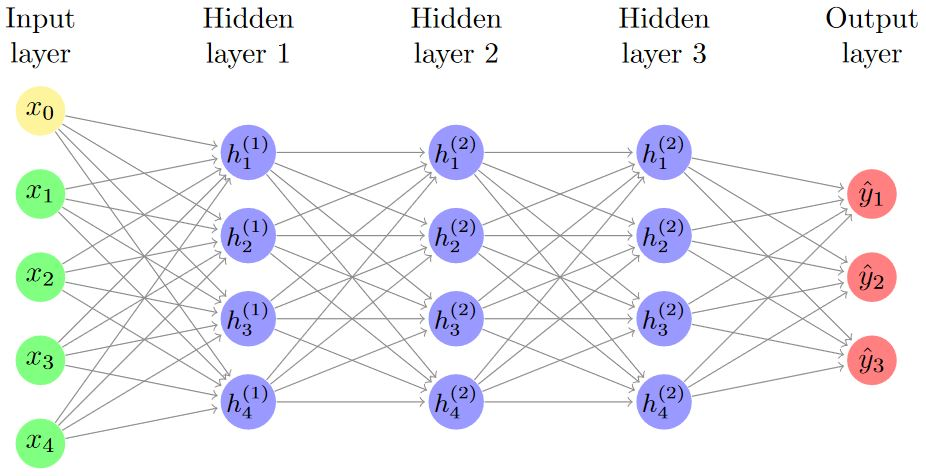
\includegraphics[scale=0.5]{Images/DFFNN.JPG}
%  \caption{Wrong! A simple Feed-forward Neural Network with 3 input neurons, 1 output neuron and 3 layers of hidden %layers consisting of 4 neurons each.$x_0$ is the bias term}
%\end{figure}

%(Write a little bit about the difference between supervised and unsupervised learning)

%\subsection{The Restricted Boltzmann Machine}
%For our Neural Network of choice, we will be implementing the Restricted Boltzmann Machine. The RBM is a Markov Random Field witch consists of a visible layer and a hidden layer where both the layers are stochastic. We will call the set of visible neurons for $\mathbf{X}$ and our set of hidden neurons for $\mathbf{H}$. Since it's restricted, there is no connection between two nodes of the same layer. In other words, there is only a connection between two nodes if one is visible whilst the other is hidden. Further, the RBM is a Generative Neural Network, which means that the weights are calibrated in order to learn a \textit{probability distribution}. We see in [\textcolor{blue}{Figure 2}] example of a RBM. 

%\newpage
%\begin{figure}[h!]
%  \centering
%  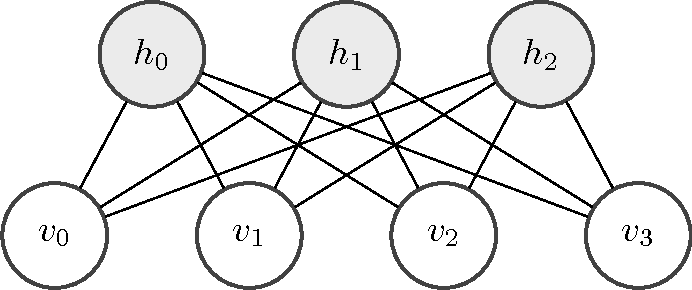
\includegraphics[scale = 0.3]{Images/RBM.png}
%  \caption{Add bunch of text here..}
%\end{figure}

%Further, the type of RBM we will use is the Gaussian/binary version. This type of RBM takes in continuous values for the visible neurons while the hidden neurons take the values either $0$ or $1$. Lastly about our RBM, since we are not working with any dataset, thus it's a Reinforcement learning algorithm, and not a supervised one. \\\\

%For the RBM, the joint probability distribution function is defined as 
%\begin{align*}
%	F_{rbm}(\mathbf{X},\mathbf{H}) = \frac{1}{Z} e^{-\frac{1}{T_0}E(\mathbf{X},\mathbf{H})}
%\end{align*}
%where $Z$ is the partition function/normalization constant given by
%\begin{align*}
%	Z = \int \int \frac{1}{Z} e^{-\frac{1}{T_0}E(\mathbf{x},\mathbf{h})} d\mathbf{x} d\mathbf{h}.
%\end{align*}
%For this project, we will set $T_0 = 1$. The function $E(\mathbf{X},\mathbf{H})$ is the energy of a configuration of nodes. What this function does is that it gives the specifics of the relation between the visible and hidden neurons. Since, we are using the Gaussian-binary RBM, our energy of a configuration of nodes is defined as, 
%\begin{align*}
%	E(\mathbf{X}, \mathbf{H}) = \sum_i^M \frac{(X_i - a_i)^2}{2\sigma_i^2} - \sum_j^N b_j H_j - \sum_{i,j}^{M,N} \frac{X_i w_{ij} H_j}{\sigma_i^2} 
%\end{align*}
%and if the term $\sigma_i = \sigma$ then
%\begin{align*}
%	E(\mathbf{X}, \mathbf{H})= \frac{||\mathbf{X} - \mathbf{a}||^2}{2\sigma^2} - \mathbf{b}^T \mathbf{H} - \frac{\mathbf{X}^T \mathbf{W} \mathbf{H}}{\sigma^2}.
%\end{align*}
%Again, the set of visible neurons is $\mathbf{X}$ and the set of hidden neurons is $\mathbf{H}$. Further, $a$ and $b$ denotes the vector of the visible and hidden biases respectively. Lastly, $\mathbf{W}$ is the matrix containing the weights which are characterizing the connection of each visible neuron to a hidden neuron. \\\\
%The only thing left now for the RBM is to find a trial wave function. The marginal distribution $P(\mathbf{X})$ is what we will use to model our wave function. We have,

%\begin{align*}
%	F_{rbm}(\mathbf{X}) &= \sum_\mathbf{h} F_{rbm}(\mathbf{X}, \mathbf{h}) \\
%				&= \frac{1}{Z}\sum_\mathbf{h} e^{-E(\mathbf{X}, \mathbf{h})}
%\end{align*}
%where $\mathbf{h}$ is....... This will be used to represent our wave function. We therefore get, 
%\begin{align*}
%\Psi (\mathbf{X}) &= P(\mathbf{X}) =  F_{rbm}(\mathbf{X})\\
%&= \frac{1}{Z}\sum_{\{h_j\}} e^{-E(\mathbf{X}, \mathbf{h})} \\
%&= \frac{1}{Z} \sum_{\{h_j\}} e^{-\sum_i^M \frac{(X_i - a_i)^2}{2\sigma^2} + \sum_j^N b_j h_j + \sum_{i,j}^{M,N} \frac{X_i w_{ij} h_j}{\sigma^2}} \\
%&= \frac{1}{Z} e^{-\sum_i^M \frac{(X_i - a_i)^2}{2\sigma^2}} \prod_j^N \left(1 + e^{b_j + \sum_i^M \frac{X_i w_{ij}}{\sigma^2}}\right) \\
%\end{align*}
%where $a_i$ and $b_i$ are elements of $a$ and $b$. With this RBM, we will be able to get a good trial wave function for us to use.

%\subsection{Hamiltonian}


\subsection{Markov Chain Monte Carlo}
Our previous project, \citep{project1}, contains informations about the theory behind our MCMC approaches. We have two approaches, the Random Walk Metropolis (RWM) and the Langevin Metropolis-Hastings (LMH). 

%\subsection{Importance sampling}
%The Metropolis-Hastings or Importance sampling.. 